\chapter{Umgestaltung des Spielkonzepts}
\label{cha:umgestaltung_spielkonzept}
Dieses Kapitel beschreibt die zu Grunde liegende Spielidee. Der Augenmerk liegt auf der Evolution der Spielmechanik, da sich basierend auf dem Ergebnis der Erhebung an der ursprünglichen Konzeption Fehleinschätzungen gezeigt haben.


\section{Ursprüngliche Konzeption}
%\label{sec:}
An dieser Stelle muss vorab gesagt werden, dass das Spiel anfangs als virtuelles Haustier geplant worden ist, die grundlegende Spielidee sich aber mit dem wachsenden Wissensstand mehr und mehr transformiert hat.
 
Diese Skizze ist eine der ersten von uns erstellten Skizzen zur Spielmechanik. Sie soll zeigen welche Features ursprünglich geplant wurden. Im Folgenden werden einzelne Punkte der Zeichnung erläutert um deren Sinn und Zweck zu klären.

Einer der wichtigsten Standpfeiler der Spielmechanik ist es, dass das Spiel nicht zeitintensiv ist. Es soll vollkommen ausreichen täglich nur einige Minuten im Spiel zu verbringen. Dies soll dabei helfen das Spielerlebnis über einen längeren Zeitraum zu vergrößern, da so die vorgegebene Story nicht einfach eben schnell innerhalb von einigen Stunden durchgespielt werden kann. Dieser Punkt hat auch die Entscheidung beeinflusst die gesamte Geschichte des Spiels Episodenbasiert zu machen. Dadurch das die Hintergrundgeschichte und das aktuelle Geschehen in Einzelteilen nachgereicht werden kann verkürzt die Zeit der Entwicklung ungemein, da alle auftauchenden Personen
an verschiedenen Orten unterschiedliche Tiere in Verschiedenen Städten 
-Diverse Boni bei Unterschiedlichen Geschäften
-Unterschiedliche Farben Items je nach Uhrzeit, Wetter, Umgebung
-Versteckte Items, Items pflanzen
-Reviere, Geofence markiert Zuhause, Tiere reagieren verschieden auf andere Tiere (Knurren, Schnuppern usw.)
-Laufweg analyse, Tiere freuen sich über neue Orte und verschiedene Geschwindigkeiten und können Spuren von anderen Tieren wahrnehmen
-Personen können Orte hinzufügen (User generated content)
-In Home Zones können die Pets ihre mobilen Endgeräte verlassen und den Rechner und andere mobile Geräte "besuchen".


\section{Alternanz des Spielkonzepts}

Wie bereits nach einigen eigenen Tests vermutet bietet der Caring-Askept nur wenig Dauermotivation. 
Nimmt man noch Tension-Release-Prinzip hinzu, fällt auf, dass dies in solchen Spielen nur an wenigen Stellen praktikabel ist.
Nun ist die Frage, wie könnte man eine Spielidee auf der neuen Basis entwickeln.
%\label{sec:}




\section{Evolution der Spieleidee} 
%\label{sec:}
Durch das Testen mehrerer Spiele, die sich mit dem Thema virtual pet beschäftigen sind wir zu dem Entschluss gekommen,  dass sich der größte teil der virtual pet spiele bzw. Lebenssimulationen einen ganz anderen Umfang als das von uns angestrebte ziel anpeilen. Wir sind ursprünglich davon ausgegangen, das die Lebenssimulationen wie bei den aus den 1990ern bekannten Tamagotchies einfach nicht optimal in die Neuzeit übertragen wurden, jedoch hat sich bei der tieferen Recherche ergeben, dass dieses genre jedoch nicht den umfang bietet ein Spiel zu entwickeln, das es schafft Spieler über einen längeren Zeitraum zu binden. Da die meisten Spieler schon nach wenigen Lebenszyklen das meiste solcher Spiele gesehen haben. Neue Items oder kleine mini Spielchen wie ein tic tac toe helfen dort auch nicht weiter. Da die Spiele damit im Grunde lediglich zu einer Minispiel-Sammlung aufgebläht werden und das eigentliche Spielprinzip dadurch mehr und mehr in den Schatten gestellt wird. Daher lag es auf der Hand das Thema von einer ganz anderen Seite her anzugehen. Wenn man das Spielkonzept durch Elemente aus rogue like game bekannten Titeln hinzufügt, erhält man plötzlich ein völlig neues und anderes Spielerlebnis.
Wie bereits im vorherigen Kapitel beschrieben, sollen Spiele, die sich nicht ihre eigene Kunst als Hauptziel setzen den Spieler fordern indem er in komplexen Situationen die bestmögliche Entscheidung treffen muss. Dies würde dazu führen, dass man nicht einfach nur sein Tier mit Nahrung versorgt, sondern darauf achten muss, was genau verfüttert wird. 
Auf der anderen Seite kann dies wiederum auch schnell frustrieren, da man auch aus Versehen das falsche Item benutzen kann und sich somit den weiteren Spielverlauf verbaut.
Ein Blick auf die finale Spiele Idee zeigt, wie sich diese Probleme umgehen lassen. 
Ein anderer Punkt ist die schnelllebige Zeit in der wir leben.





\section{Neue Basisidee} 
%\label{sec:}
Es soll ein einfach erlernbares Spiel entwickelt werden, das den Spieler immer wieder vor Entscheidungen stellen soll, die ihn zum Nachdenken anregen sollen.


\section{Definition der Spielmechanik} 
%\label{sec:}
Die neue Grundidee des Spiels ist es verschiedene nach wie vor verschiedene Tiere zu fangen, jedoch ist die Lebensdauer eines Tiers stark beschränkt. Die Hauptresource die dem Spieler zur Verfügung steht ist Zeit. Dies soll dazu beitragen, das die Spieler sich genau überlegen wie sie mit der Zeit umgehen wollen. Durch die neuen Items, wird dieser Aspekt noch weiter gestärkt, denn keines der Items soll nur Vorteile bringen. Somit muss sich der Spieler bei jedem Gegenstand genau überlegen, ob er es wirklich einsetzen möchte. Dies ist ein ganz wichtiger Punkt. Denn jede Entscheidung des Spielers soll einen großen Einfluss auf das gesamte Spielgeschehen haben. Somit besteht die Hauptaufgabe darin, mit seinem Tier in 7 Tagen möglichst viele Punkte, die im weiteren Verlauf auch Victory Points genannt werden oder mit VP abgekürzt werden, zu sammeln. Diese kann der Spieler durch gewonnen Kämpfe erhalten oder jeweils einen für jede Minute, die sein Tier am Leben ist. 
Das fangen der Tiere gestaltet sich so, dass dem Spieler einfach durch drücken des Tier aufspüren Knopfes ein neues Tier generiert wird. Dieser Vorgang lässt sich natürlich noch weiter ausschmücken, indem man vielleicht ein kleines minispiel hinzufügt, mit dem man das tier an sich gewöhnen muss. Das gefangene Tier unterscheidet sich je nach Standort. so wird die Farbe je nach Tageszeit und Ort. 
Hat mein ein tier gefangen, wird man dazu aufgefordert ein Revier für sein tier zu markieren. Reviere sind die gebiete, in denen die Tiere "außerhalb" des telefons leben. Es ist so zu verstehen, das ein Tier in einem Revier verweilt und mittels des Spiels eine Verbindung dazu hergestellt wird. Außerdem sind Reviere interaktive Gebiete. Ein Spieler kann jedoch nur ein Revier selber erstellen. Er kann aber mehrere Reviere erspielen, indem er andere Spieler besiegt und deren Reviere für sich beansprucht. Des weiteren werden alle Reviere in der aktuellen Umgebung des Spielers auf der Karte im Spiel angezeigt. Somit kann ein Spieler sich auf der Karte ein Revier aussuchen, sich dorthin begeben und dieses nach einem erfolgreichen Kampf für sich beanspruchen. Zum markieren des Reviers gehört zudem einen Wert des eigenen Tieres auszuwählen, mit dem es Kämpft. Daher wird nun erst etwas genauer auf das Kampfsystem eingegangen. Die Basis das Kampfsystems besteht auf einer erweiterten Version des alt bekannten Spiels, Schere, Stein, Papier und wird um 2 weiter Punkte erweitert. Die neuen Werte sind Stärke, Intelligenz, Geschicklichkeit, Charisma, Glück.



Die Abbildung zeigt, wie die Werte gegeneinander aufgestellt sind. Somit schlägt zum Beispiel Intelligenz Stärke aber würde jedoch von Geschick selber geschlagen. Zu diesem recht einfachen Prinzip kommt aber noch ein Werte-System hinzu. Beim Fangen bzw. der Erstellung eines Tieres, werden die Werte zufällig zwischen 1 und 100 für jedes einzelne Attribut gewählt. Auf dem Server befindet sich zudem eine Tabelle, die für bestimmte Tiere bonus werte erhält. So kann man im weiteren Verlauf Gebiete definieren in denen beim Fangen ein Bonuswert von zum Beispiel 10 oder mehr Punkten gewährt wird.

%Somit könnte Tier A so aussehen:
%
%Stärke    Intelligenz    Geschick    Charisma    Glück
%44        65             74          89          12
%
%Und Tier B so:
%Stärke    Intelligenz    Geschick    Charisma    Glück
%55        94             70          61          49


Durch die Werte bei den Attributen wird nun nicht mehr direkt geschlagen, sondern ein Bonus verteilt. Würde wie in der Abbildung Monster A Monster B mit dem Stärke Attribut angreifen, und der Besitzer von Monster B Geschick als Attribut wählen, würde Monster A einen Bonus von 50 Punkten auf sein Attribut erhalten und somit Monster B besiegen. Nach dem Sieg werden die Victory Points vergeben. Der Besitzer von Monster A erhält nun entsprechend der Anzahl an Spielen, die er am aktuellen Tag getätigt hat.
Die lässt sich am folgenden Graphen zeigen:

\textbf{Victory Points:}

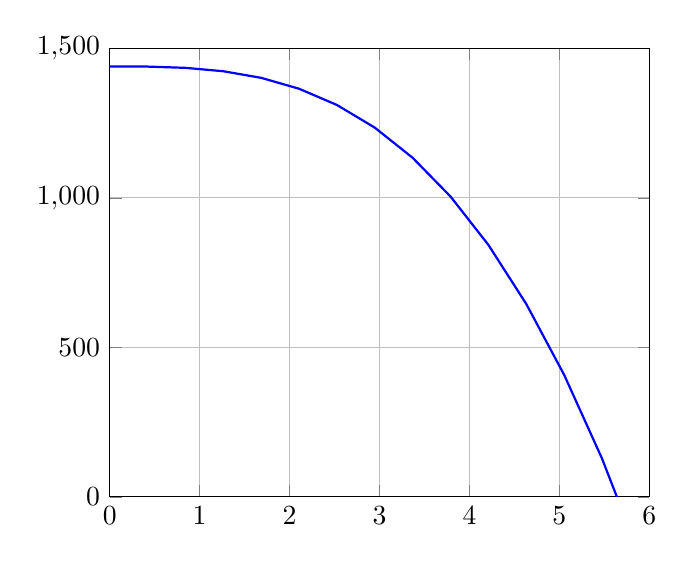
\begin{tikzpicture}
\begin{axis}[domain=0:8,
    samples=20,
    xmin=0,   xmax=6,
    ymin=0,   ymax=1500,
    grid=both, no markers
  ]
\addplot +[thick] {(-8*(x^3))+1440};
\end{axis}
\end{tikzpicture}

Die Formel für die VP lässt sich so berechnen: $(-8*(x^3))+1440$. 
Daraus ergibt sich, dass der erste Sieg an einem Tag 1044 VP dem Spieler einbringt. Für einen weiteren Sieg würde er nur noch 1432 Punkte erhalten. Dies läuft solange weiter, bis man nach dem fünften Sieg nur noch 440 Punkte erhält. Ein sechster Sieg würde weiterhin 440 Punkte bringen. Dies hat zur Folge, dass Spieler die sehr viel Spielen nicht viel mehr Punkte bekommen, als Spieler die am Tag nur 2-3 Runden Spielen können. Es gibt aber weiterhin so viele Punkte das es sich auch lohnt weitere Runden zu spielen um einen höheren Highscore zu erreichen. 

1440, 1432, 1376, 1224, 440

Ziel des Spiels ist es einen möglichst hohen Highscore zu erreichen, dadurch können die Spieler auf einer Liste vergleichen, wie gut sich im Gegensatz zu anderen Spielern abschneiden. Der Highscore setzt sich zusammen aus der Lebenszeit, die das Tier überlebt hat und den victory points, welche der spieler durch das erzielen von siegen erhält. Dies geschieht durch eine einfache Addition, Lebenszeit (in Minuten) + Victory Points).
Um den Highscore leichter lesbar als in vielen anderen Spielen zu machen wird die Lebenszeit in Minuten gemessen, was auch den Vorteil bringt, das sie zeitkritisch ist, aber trotzdem relativ genau ist.
Der maximale Puntkestand, den man ohne Kämpfe erreichen kann ist daher MaxLebenszeit: (7*24*60 = 10080) und ist die Anzahl der Minuten, die eine Woche hat. 
Dies soll auch als Referenzwert dienen, da man ihn leicht überschreiten kann aber auch durch einige Fehlentscheidungen auch unterschreiten kann.

Um die Kämpfe und den gesamten Spielablauf spannender zu gestalten, kann Spieler Items einzusetzen. 
Die folgende Tablle zeigt, welche Items welchen Bonus bringen.
Stärke – Strength:		Hantel\\
Intelligenz – Intelligence: 		Buch\\
Geschicklichkeit – Dexterity:	Werkzeug\\
Charisma – Charisma:		Spiegel\\
Glück – Luck:				Kleeblatt \\
Obwohl diese standard Items, von Begin für den Spieler verfügbar sind, können sie jedoch nicht beliebig eingesetzt werden. Wird ein Gegenstand eingesetzt, muss der Spieler einen Tag der Lebenszeit seines Tieres dafür bezahlen. Zudem können die Gegenstände auch nicht beliebig oft eingesetzt werden. Benutzt man das erste mal einen Gegenstand, erhält das Tier +50 Punkte auf den gewünschten wert. Wird ein zweites Item eingesetzt, werden nur noch 25 Punkte gutgeschrieben. Die Punkte werden so lange reduziert, bis ein Item nur noch 7 Punkte auf den jeweiligen Wert addiert. Die Punkte werden also in jedem Schritt halbiert und danach aufgerundet. 
Items: +50,  +25, +13, +7

Die Kämpfe laufen wie folgt ab. Nachdem ein Spieler das Revier von einem anderen Spieler bzw. Tieres betritt während das Spiel auf dem Telefon läuft, kann er einen der oben genannten Werte auswählen, wie z.B. Stärke oder Intelligenz. Mit diesem Wert wird dann das andere Tier in seinem Revier angegriffen und verteidigt sich mit dem Wert, den der andere Spieler zuvor gewählt hat. Sollte es nach Berechnung des Bonus trotzdem zu einem Unentschieden kommen, gewinnt das Tier, das älter ist. Dies bedeutet, das es so gut wie gar nicht zu einem Unentschieden kommen kann, da nicht nur die Werte identisch sein müssten, sondern auch die Sekunde, in der beide Tiere gefangen wurden. Zudem soll es nicht möglich sein ein Revier mehrmals an einem Tag zu betreten. Dadurch soll verhindert werden, dass ein Spieler, nachdem er herausgefunden hat, mit welchem Wert er am besten antritt, dies andauernd wiederholt um schnell viele Punkte zu erreichen. Dies hat zudem den Vorteil, das die Spieler sich weiter bewegen müssen um Kämpfe zu bestreiten. Des Weiteren werden auch trotz einer Niederlage keine Punkte abgezogen. 

Um das Kampfgeschehen nicht zu stark vorhersehbar zu machen, werden dem Spieler die Werte des eigenen Tieres nicht angezeigt. Sondern erst nach und nach zufällig aufgedeckt. Es wird jeden Tag ein neuer Wert angezeigt. Somit erhält der Spieler jeden Tag eine Information mehr über sein Tier.

